\section{Delaunay triangulation}
\label{sec:triangulation}

We describe two common algorithms for generated a Delaunay triangulation of a given set of points.
Both algorithms are incremental.

\subsection{Bowyer-Watson}
\label{sub:bowyer_watson}

\begin{figure}
    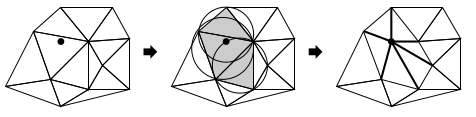
\includegraphics[width=\columnwidth]{../images/BW.png}
    \caption{Demonstration of Bowyer-Watson}
\end{figure}

The Bowyer-Watson (B-W) algorithm was independently introduced by Bowyer \cite{art:Bowyer1981} and Watson \cite{art:Watson1981} in 1981.
When incrementally inserting a vertex, B-W removes all triangles that violate the Delaunay property after insertion of the new vertex.
Then, the boundary of the created cavity is connected to the new vertex, which results in a new Delaunay triangulation.
%TODO: see figure . . .
This algorithm has an expected runtime of $O(n)$ \cite{shewchuk}.

\begin{algorithm}
    \caption{Bowyer/Watson}
    \begin{algorithmic}
        \Function{Triangulate}{$P$}
            \State{Initialize $T$ with a single large triangle in which all vertices of $P$ are contained}
            \ForAll{$p \in P$}
                \State{Let $T'$ be the set of all triangles in $T$ whose circumcircle contains $p$}
                \State{Remove triangles in $T'$ from $T$}
                \State{Find the total boundary, $B$, of the triangles in $T'$}
                \State{For each edge $e \in B$, create the triangle connecting $e$ to $p$ and add it to $T$}
            \EndFor
            \State{Remove the initial triangle \\}
            \Return $D$ = $T$, the Delaunay Triangulation of $P$
        \EndFunction
    \end{algorithmic}
\end{algorithm}

The Bowyer-Watson algorithm can be extended to create a constrained Delaunay triangulation.
In this case, the segments connecting $p$ and each of the edges of the boundary, $B$, may not
intersect with any segment in the PSLG.
Ultimately, this boils down to having to check for each PSLG edge in the cavity, $T'$, if this condition is violated.
If violated, then the adjacent triangle (the one distant from $p$) should not be added to the cavity.
By keeping a list of all PSLG edges and checking whether a to-be-checked edge is in the PSLG this may be implemented relatively cheaply.
Though, the algorithm adaptation is more complicated than for Lawson's algorithm.

\subsection{Lawson}
\label{sub:lawson}
Lawson's algorithm makes use of the principle of edge-flips.
A theorem states that ``either two triangles are both locally Delaunay or their common edge may be flipped
and the result is two locally Delaunay triangles''.
Here, `locally Delaunay' is defined as `Delaunay', while only taking these two triangles into account.
Lawson's algorithm is easily implemented in 2 dimensions, but is harder to generalize to more dimensions.
This algorithm has an expected runtime of $O(n)$ \cite{shewchuk}.

\begin{figure}
    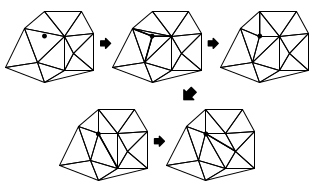
\includegraphics[width=\columnwidth]{../images/Lawson.png}
    \caption{Demonstration of Lawson}
\end{figure}

\begin{algorithm}
    \caption{Lawson}
    \begin{algorithmic}
        \Function{Triangulate}{$P$}
            \State{Initialize $T$ with a single large triangle in which all vertices of $P$ are contained}
            \ForAll{$p \in P$}
                \State{Locate the triangle $t$ that contains $p$ and connect the edges of $t$ to $p$ creating 3 new triangles, $T'$}
                \State{Remove $t$ from $T$ and add $T'$ to T}
                \State{Call Edge-flip on the three edges in $T'$ that do not contain $p$.}
            \EndFor
            \State{Remove the initial triangle\\}
            \Return $D$ = $T$, the Delaunay Triangulation of $P$
        \EndFunction
        \Function{Edge-flip}{edge $e$}
            \If{$e$ is not locally Delaunay}
                \State{Flip $e$ to replace the two adjacent triangles with two new triangles}
                \State{Call Edge-Flip on all outer edges of the two adjacent triangles}
            \EndIf
        \EndFunction
    \end{algorithmic}
\end{algorithm}

Lawson's algorithm can be extended to create a constrained Delaunay triangulation.
To do so, we must append the if-statement of the edge-flip function by the condition that $e$ is not in the PSLG.
Also, the initial triangulation, $T$, should not violate the PSLG.

%A worst case analysis can be done by backward analysis.
%When we have a correct triangulation, we consider choosing a random vertex and removing that vertex from the triangulation.

%\begin{algorithm}
  %\caption{Counting mismatches between two packed \DNA strings
    %\label{alg:packed-dna-hamming}}
  %\begin{algorithmic}[1]
    %\Require{$x$ and $y$ are packed \DNA strings of equal length $n$}
    %\Statex
    %\Function{Distance}{$x, y$}
      %\Let{$z$}{$x \oplus y$} \Comment{$\oplus$: bitwise exclusive-or}
      %\Let{$\delta$}{$0$}
      %\For{$i \gets 1 \textrm{ to } n$}
        %\If{$z_i \neq 0$}
          %\Let{$\delta$}{$\delta + 1$}
        %\EndIf
      %\EndFor
      %\State \Return{$\delta$}
    %\EndFunction
  %\end{algorithmic}
%\end{algorithm}

